% Created by tikzDevice version 0.12.3.1 on 2022-01-03 22:16:31
% !TEX encoding = UTF-8 Unicode
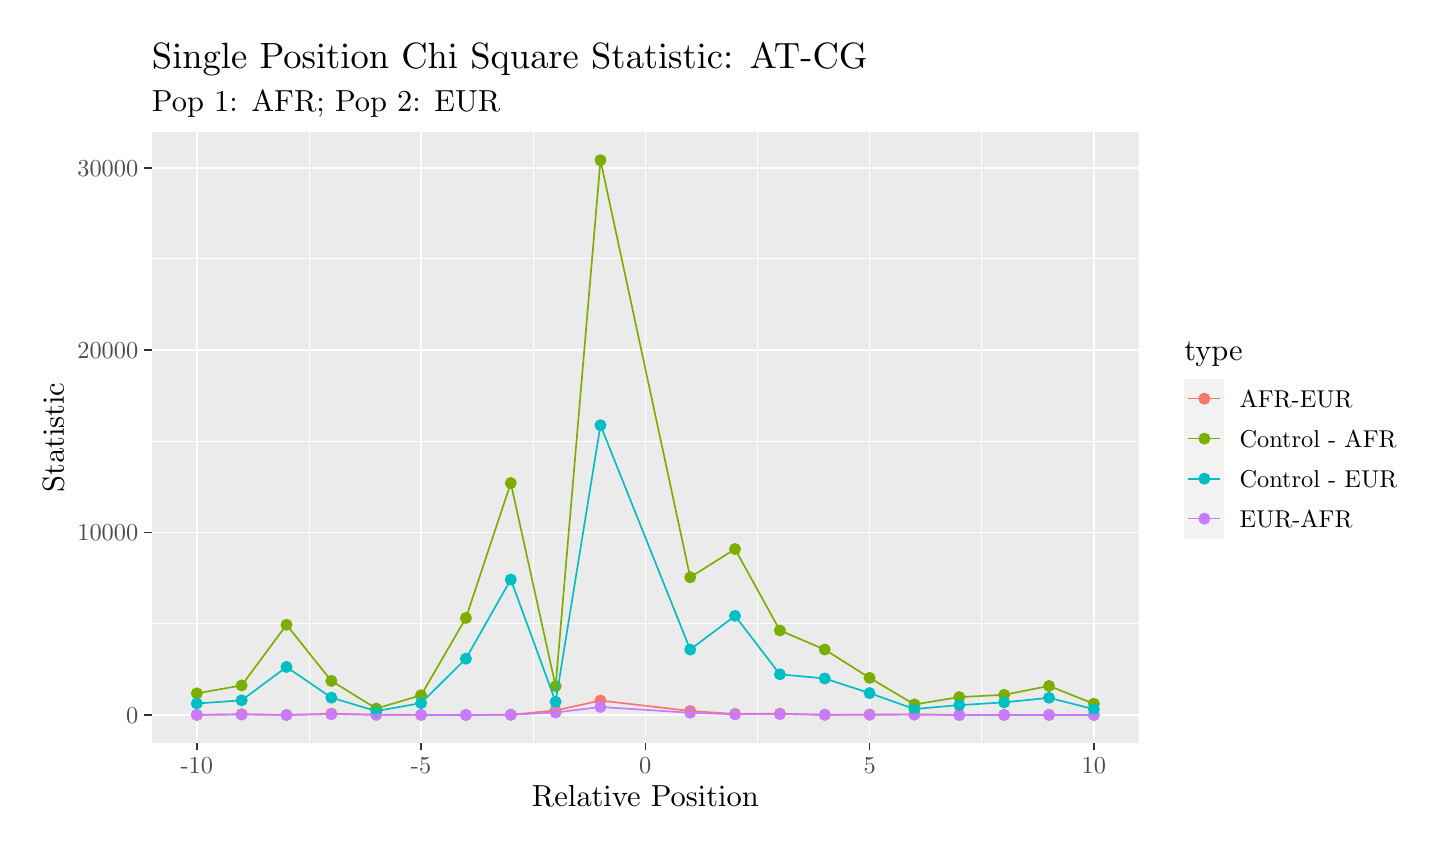
\begin{tikzpicture}[x=1pt,y=1pt]
\definecolor{fillColor}{RGB}{255,255,255}
\path[use as bounding box,fill=fillColor,fill opacity=0.00] (0,0) rectangle (505.89,289.08);
\begin{scope}
\path[clip] (  0.00,  0.00) rectangle (505.89,289.08);
\definecolor{drawColor}{RGB}{255,255,255}
\definecolor{fillColor}{RGB}{255,255,255}

\path[draw=drawColor,line width= 0.6pt,line join=round,line cap=round,fill=fillColor] (  0.00,  0.00) rectangle (505.89,289.08);
\end{scope}
\begin{scope}
\path[clip] ( 44.91, 30.69) rectangle (401.47,251.21);
\definecolor{fillColor}{gray}{0.92}

\path[fill=fillColor] ( 44.91, 30.69) rectangle (401.47,251.21);
\definecolor{drawColor}{RGB}{255,255,255}

\path[draw=drawColor,line width= 0.3pt,line join=round] ( 44.91, 73.67) --
	(401.47, 73.67);

\path[draw=drawColor,line width= 0.3pt,line join=round] ( 44.91,139.59) --
	(401.47,139.59);

\path[draw=drawColor,line width= 0.3pt,line join=round] ( 44.91,205.52) --
	(401.47,205.52);

\path[draw=drawColor,line width= 0.3pt,line join=round] (101.63, 30.69) --
	(101.63,251.21);

\path[draw=drawColor,line width= 0.3pt,line join=round] (182.67, 30.69) --
	(182.67,251.21);

\path[draw=drawColor,line width= 0.3pt,line join=round] (263.71, 30.69) --
	(263.71,251.21);

\path[draw=drawColor,line width= 0.3pt,line join=round] (344.74, 30.69) --
	(344.74,251.21);

\path[draw=drawColor,line width= 0.6pt,line join=round] ( 44.91, 40.71) --
	(401.47, 40.71);

\path[draw=drawColor,line width= 0.6pt,line join=round] ( 44.91,106.63) --
	(401.47,106.63);

\path[draw=drawColor,line width= 0.6pt,line join=round] ( 44.91,172.56) --
	(401.47,172.56);

\path[draw=drawColor,line width= 0.6pt,line join=round] ( 44.91,238.48) --
	(401.47,238.48);

\path[draw=drawColor,line width= 0.6pt,line join=round] ( 61.12, 30.69) --
	( 61.12,251.21);

\path[draw=drawColor,line width= 0.6pt,line join=round] (142.15, 30.69) --
	(142.15,251.21);

\path[draw=drawColor,line width= 0.6pt,line join=round] (223.19, 30.69) --
	(223.19,251.21);

\path[draw=drawColor,line width= 0.6pt,line join=round] (304.23, 30.69) --
	(304.23,251.21);

\path[draw=drawColor,line width= 0.6pt,line join=round] (385.26, 30.69) --
	(385.26,251.21);
\definecolor{drawColor}{RGB}{248,118,109}
\definecolor{fillColor}{RGB}{248,118,109}

\path[draw=drawColor,line width= 0.4pt,line join=round,line cap=round,fill=fillColor] ( 61.12, 40.76) circle (  1.96);

\path[draw=drawColor,line width= 0.4pt,line join=round,line cap=round,fill=fillColor] ( 77.32, 41.00) circle (  1.96);

\path[draw=drawColor,line width= 0.4pt,line join=round,line cap=round,fill=fillColor] ( 93.53, 40.73) circle (  1.96);

\path[draw=drawColor,line width= 0.4pt,line join=round,line cap=round,fill=fillColor] (109.74, 41.18) circle (  1.96);

\path[draw=drawColor,line width= 0.4pt,line join=round,line cap=round,fill=fillColor] (125.95, 40.83) circle (  1.96);

\path[draw=drawColor,line width= 0.4pt,line join=round,line cap=round,fill=fillColor] (142.15, 40.76) circle (  1.96);

\path[draw=drawColor,line width= 0.4pt,line join=round,line cap=round,fill=fillColor] (158.36, 40.73) circle (  1.96);

\path[draw=drawColor,line width= 0.4pt,line join=round,line cap=round,fill=fillColor] (174.57, 40.82) circle (  1.96);

\path[draw=drawColor,line width= 0.4pt,line join=round,line cap=round,fill=fillColor] (190.77, 42.35) circle (  1.96);

\path[draw=drawColor,line width= 0.4pt,line join=round,line cap=round,fill=fillColor] (206.98, 45.94) circle (  1.96);

\path[draw=drawColor,line width= 0.4pt,line join=round,line cap=round,fill=fillColor] (239.40, 42.16) circle (  1.96);

\path[draw=drawColor,line width= 0.4pt,line join=round,line cap=round,fill=fillColor] (255.60, 41.12) circle (  1.96);

\path[draw=drawColor,line width= 0.4pt,line join=round,line cap=round,fill=fillColor] (271.81, 41.20) circle (  1.96);

\path[draw=drawColor,line width= 0.4pt,line join=round,line cap=round,fill=fillColor] (288.02, 40.81) circle (  1.96);

\path[draw=drawColor,line width= 0.4pt,line join=round,line cap=round,fill=fillColor] (304.23, 40.87) circle (  1.96);

\path[draw=drawColor,line width= 0.4pt,line join=round,line cap=round,fill=fillColor] (320.43, 40.96) circle (  1.96);

\path[draw=drawColor,line width= 0.4pt,line join=round,line cap=round,fill=fillColor] (336.64, 40.71) circle (  1.96);

\path[draw=drawColor,line width= 0.4pt,line join=round,line cap=round,fill=fillColor] (352.85, 40.72) circle (  1.96);

\path[draw=drawColor,line width= 0.4pt,line join=round,line cap=round,fill=fillColor] (369.06, 40.77) circle (  1.96);

\path[draw=drawColor,line width= 0.4pt,line join=round,line cap=round,fill=fillColor] (385.26, 40.74) circle (  1.96);
\definecolor{drawColor}{RGB}{199,124,255}
\definecolor{fillColor}{RGB}{199,124,255}

\path[draw=drawColor,line width= 0.4pt,line join=round,line cap=round,fill=fillColor] ( 61.12, 40.74) circle (  1.96);

\path[draw=drawColor,line width= 0.4pt,line join=round,line cap=round,fill=fillColor] ( 77.32, 40.88) circle (  1.96);

\path[draw=drawColor,line width= 0.4pt,line join=round,line cap=round,fill=fillColor] ( 93.53, 40.72) circle (  1.96);

\path[draw=drawColor,line width= 0.4pt,line join=round,line cap=round,fill=fillColor] (109.74, 40.98) circle (  1.96);

\path[draw=drawColor,line width= 0.4pt,line join=round,line cap=round,fill=fillColor] (125.95, 40.78) circle (  1.96);

\path[draw=drawColor,line width= 0.4pt,line join=round,line cap=round,fill=fillColor] (142.15, 40.74) circle (  1.96);

\path[draw=drawColor,line width= 0.4pt,line join=round,line cap=round,fill=fillColor] (158.36, 40.72) circle (  1.96);

\path[draw=drawColor,line width= 0.4pt,line join=round,line cap=round,fill=fillColor] (174.57, 40.77) circle (  1.96);

\path[draw=drawColor,line width= 0.4pt,line join=round,line cap=round,fill=fillColor] (190.77, 41.62) circle (  1.96);

\path[draw=drawColor,line width= 0.4pt,line join=round,line cap=round,fill=fillColor] (206.98, 43.62) circle (  1.96);

\path[draw=drawColor,line width= 0.4pt,line join=round,line cap=round,fill=fillColor] (239.40, 41.52) circle (  1.96);

\path[draw=drawColor,line width= 0.4pt,line join=round,line cap=round,fill=fillColor] (255.60, 40.94) circle (  1.96);

\path[draw=drawColor,line width= 0.4pt,line join=round,line cap=round,fill=fillColor] (271.81, 40.99) circle (  1.96);

\path[draw=drawColor,line width= 0.4pt,line join=round,line cap=round,fill=fillColor] (288.02, 40.76) circle (  1.96);

\path[draw=drawColor,line width= 0.4pt,line join=round,line cap=round,fill=fillColor] (304.23, 40.80) circle (  1.96);

\path[draw=drawColor,line width= 0.4pt,line join=round,line cap=round,fill=fillColor] (320.43, 40.85) circle (  1.96);

\path[draw=drawColor,line width= 0.4pt,line join=round,line cap=round,fill=fillColor] (336.64, 40.71) circle (  1.96);

\path[draw=drawColor,line width= 0.4pt,line join=round,line cap=round,fill=fillColor] (352.85, 40.71) circle (  1.96);

\path[draw=drawColor,line width= 0.4pt,line join=round,line cap=round,fill=fillColor] (369.06, 40.74) circle (  1.96);

\path[draw=drawColor,line width= 0.4pt,line join=round,line cap=round,fill=fillColor] (385.26, 40.73) circle (  1.96);
\definecolor{drawColor}{RGB}{124,174,0}
\definecolor{fillColor}{RGB}{124,174,0}

\path[draw=drawColor,line width= 0.4pt,line join=round,line cap=round,fill=fillColor] ( 61.12, 48.53) circle (  1.96);

\path[draw=drawColor,line width= 0.4pt,line join=round,line cap=round,fill=fillColor] ( 77.32, 51.40) circle (  1.96);

\path[draw=drawColor,line width= 0.4pt,line join=round,line cap=round,fill=fillColor] ( 93.53, 73.32) circle (  1.96);

\path[draw=drawColor,line width= 0.4pt,line join=round,line cap=round,fill=fillColor] (109.74, 53.04) circle (  1.96);

\path[draw=drawColor,line width= 0.4pt,line join=round,line cap=round,fill=fillColor] (125.95, 43.05) circle (  1.96);

\path[draw=drawColor,line width= 0.4pt,line join=round,line cap=round,fill=fillColor] (142.15, 47.85) circle (  1.96);

\path[draw=drawColor,line width= 0.4pt,line join=round,line cap=round,fill=fillColor] (158.36, 75.77) circle (  1.96);

\path[draw=drawColor,line width= 0.4pt,line join=round,line cap=round,fill=fillColor] (174.57,124.53) circle (  1.96);

\path[draw=drawColor,line width= 0.4pt,line join=round,line cap=round,fill=fillColor] (190.77, 51.13) circle (  1.96);

\path[draw=drawColor,line width= 0.4pt,line join=round,line cap=round,fill=fillColor] (206.98,241.18) circle (  1.96);

\path[draw=drawColor,line width= 0.4pt,line join=round,line cap=round,fill=fillColor] (239.40, 90.47) circle (  1.96);

\path[draw=drawColor,line width= 0.4pt,line join=round,line cap=round,fill=fillColor] (255.60,100.68) circle (  1.96);

\path[draw=drawColor,line width= 0.4pt,line join=round,line cap=round,fill=fillColor] (271.81, 71.27) circle (  1.96);

\path[draw=drawColor,line width= 0.4pt,line join=round,line cap=round,fill=fillColor] (288.02, 64.37) circle (  1.96);

\path[draw=drawColor,line width= 0.4pt,line join=round,line cap=round,fill=fillColor] (304.23, 54.13) circle (  1.96);

\path[draw=drawColor,line width= 0.4pt,line join=round,line cap=round,fill=fillColor] (320.43, 44.54) circle (  1.96);

\path[draw=drawColor,line width= 0.4pt,line join=round,line cap=round,fill=fillColor] (336.64, 47.18) circle (  1.96);

\path[draw=drawColor,line width= 0.4pt,line join=round,line cap=round,fill=fillColor] (352.85, 48.00) circle (  1.96);

\path[draw=drawColor,line width= 0.4pt,line join=round,line cap=round,fill=fillColor] (369.06, 51.21) circle (  1.96);

\path[draw=drawColor,line width= 0.4pt,line join=round,line cap=round,fill=fillColor] (385.26, 44.78) circle (  1.96);
\definecolor{drawColor}{RGB}{0,191,196}
\definecolor{fillColor}{RGB}{0,191,196}

\path[draw=drawColor,line width= 0.4pt,line join=round,line cap=round,fill=fillColor] ( 61.12, 44.87) circle (  1.96);

\path[draw=drawColor,line width= 0.4pt,line join=round,line cap=round,fill=fillColor] ( 77.32, 46.01) circle (  1.96);

\path[draw=drawColor,line width= 0.4pt,line join=round,line cap=round,fill=fillColor] ( 93.53, 58.07) circle (  1.96);

\path[draw=drawColor,line width= 0.4pt,line join=round,line cap=round,fill=fillColor] (109.74, 46.98) circle (  1.96);

\path[draw=drawColor,line width= 0.4pt,line join=round,line cap=round,fill=fillColor] (125.95, 42.14) circle (  1.96);

\path[draw=drawColor,line width= 0.4pt,line join=round,line cap=round,fill=fillColor] (142.15, 45.01) circle (  1.96);

\path[draw=drawColor,line width= 0.4pt,line join=round,line cap=round,fill=fillColor] (158.36, 61.07) circle (  1.96);

\path[draw=drawColor,line width= 0.4pt,line join=round,line cap=round,fill=fillColor] (174.57, 89.68) circle (  1.96);

\path[draw=drawColor,line width= 0.4pt,line join=round,line cap=round,fill=fillColor] (190.77, 45.49) circle (  1.96);

\path[draw=drawColor,line width= 0.4pt,line join=round,line cap=round,fill=fillColor] (206.98,145.43) circle (  1.96);

\path[draw=drawColor,line width= 0.4pt,line join=round,line cap=round,fill=fillColor] (239.40, 64.35) circle (  1.96);

\path[draw=drawColor,line width= 0.4pt,line join=round,line cap=round,fill=fillColor] (255.60, 76.54) circle (  1.96);

\path[draw=drawColor,line width= 0.4pt,line join=round,line cap=round,fill=fillColor] (271.81, 55.41) circle (  1.96);

\path[draw=drawColor,line width= 0.4pt,line join=round,line cap=round,fill=fillColor] (288.02, 53.91) circle (  1.96);

\path[draw=drawColor,line width= 0.4pt,line join=round,line cap=round,fill=fillColor] (304.23, 48.62) circle (  1.96);

\path[draw=drawColor,line width= 0.4pt,line join=round,line cap=round,fill=fillColor] (320.43, 42.88) circle (  1.96);

\path[draw=drawColor,line width= 0.4pt,line join=round,line cap=round,fill=fillColor] (336.64, 44.29) circle (  1.96);

\path[draw=drawColor,line width= 0.4pt,line join=round,line cap=round,fill=fillColor] (352.85, 45.27) circle (  1.96);

\path[draw=drawColor,line width= 0.4pt,line join=round,line cap=round,fill=fillColor] (369.06, 46.93) circle (  1.96);

\path[draw=drawColor,line width= 0.4pt,line join=round,line cap=round,fill=fillColor] (385.26, 42.82) circle (  1.96);
\definecolor{drawColor}{RGB}{248,118,109}

\path[draw=drawColor,line width= 0.6pt,line join=round] ( 61.12, 40.76) --
	( 77.32, 41.00) --
	( 93.53, 40.73) --
	(109.74, 41.18) --
	(125.95, 40.83) --
	(142.15, 40.76) --
	(158.36, 40.73) --
	(174.57, 40.82) --
	(190.77, 42.35) --
	(206.98, 45.94) --
	(239.40, 42.16) --
	(255.60, 41.12) --
	(271.81, 41.20) --
	(288.02, 40.81) --
	(304.23, 40.87) --
	(320.43, 40.96) --
	(336.64, 40.71) --
	(352.85, 40.72) --
	(369.06, 40.77) --
	(385.26, 40.74);
\definecolor{drawColor}{RGB}{124,174,0}

\path[draw=drawColor,line width= 0.6pt,line join=round] ( 61.12, 48.53) --
	( 77.32, 51.40) --
	( 93.53, 73.32) --
	(109.74, 53.04) --
	(125.95, 43.05) --
	(142.15, 47.85) --
	(158.36, 75.77) --
	(174.57,124.53) --
	(190.77, 51.13) --
	(206.98,241.18) --
	(239.40, 90.47) --
	(255.60,100.68) --
	(271.81, 71.27) --
	(288.02, 64.37) --
	(304.23, 54.13) --
	(320.43, 44.54) --
	(336.64, 47.18) --
	(352.85, 48.00) --
	(369.06, 51.21) --
	(385.26, 44.78);
\definecolor{drawColor}{RGB}{0,191,196}

\path[draw=drawColor,line width= 0.6pt,line join=round] ( 61.12, 44.87) --
	( 77.32, 46.01) --
	( 93.53, 58.07) --
	(109.74, 46.98) --
	(125.95, 42.14) --
	(142.15, 45.01) --
	(158.36, 61.07) --
	(174.57, 89.68) --
	(190.77, 45.49) --
	(206.98,145.43) --
	(239.40, 64.35) --
	(255.60, 76.54) --
	(271.81, 55.41) --
	(288.02, 53.91) --
	(304.23, 48.62) --
	(320.43, 42.88) --
	(336.64, 44.29) --
	(352.85, 45.27) --
	(369.06, 46.93) --
	(385.26, 42.82);
\definecolor{drawColor}{RGB}{199,124,255}

\path[draw=drawColor,line width= 0.6pt,line join=round] ( 61.12, 40.74) --
	( 77.32, 40.88) --
	( 93.53, 40.72) --
	(109.74, 40.98) --
	(125.95, 40.78) --
	(142.15, 40.74) --
	(158.36, 40.72) --
	(174.57, 40.77) --
	(190.77, 41.62) --
	(206.98, 43.62) --
	(239.40, 41.52) --
	(255.60, 40.94) --
	(271.81, 40.99) --
	(288.02, 40.76) --
	(304.23, 40.80) --
	(320.43, 40.85) --
	(336.64, 40.71) --
	(352.85, 40.71) --
	(369.06, 40.74) --
	(385.26, 40.73);
\end{scope}
\begin{scope}
\path[clip] (  0.00,  0.00) rectangle (505.89,289.08);
\definecolor{drawColor}{gray}{0.30}

\node[text=drawColor,anchor=base east,inner sep=0pt, outer sep=0pt, scale=  0.88] at ( 39.96, 37.68) {0};

\node[text=drawColor,anchor=base east,inner sep=0pt, outer sep=0pt, scale=  0.88] at ( 39.96,103.60) {10000};

\node[text=drawColor,anchor=base east,inner sep=0pt, outer sep=0pt, scale=  0.88] at ( 39.96,169.53) {20000};

\node[text=drawColor,anchor=base east,inner sep=0pt, outer sep=0pt, scale=  0.88] at ( 39.96,235.45) {30000};
\end{scope}
\begin{scope}
\path[clip] (  0.00,  0.00) rectangle (505.89,289.08);
\definecolor{drawColor}{gray}{0.20}

\path[draw=drawColor,line width= 0.6pt,line join=round] ( 42.16, 40.71) --
	( 44.91, 40.71);

\path[draw=drawColor,line width= 0.6pt,line join=round] ( 42.16,106.63) --
	( 44.91,106.63);

\path[draw=drawColor,line width= 0.6pt,line join=round] ( 42.16,172.56) --
	( 44.91,172.56);

\path[draw=drawColor,line width= 0.6pt,line join=round] ( 42.16,238.48) --
	( 44.91,238.48);
\end{scope}
\begin{scope}
\path[clip] (  0.00,  0.00) rectangle (505.89,289.08);
\definecolor{drawColor}{gray}{0.20}

\path[draw=drawColor,line width= 0.6pt,line join=round] ( 61.12, 27.94) --
	( 61.12, 30.69);

\path[draw=drawColor,line width= 0.6pt,line join=round] (142.15, 27.94) --
	(142.15, 30.69);

\path[draw=drawColor,line width= 0.6pt,line join=round] (223.19, 27.94) --
	(223.19, 30.69);

\path[draw=drawColor,line width= 0.6pt,line join=round] (304.23, 27.94) --
	(304.23, 30.69);

\path[draw=drawColor,line width= 0.6pt,line join=round] (385.26, 27.94) --
	(385.26, 30.69);
\end{scope}
\begin{scope}
\path[clip] (  0.00,  0.00) rectangle (505.89,289.08);
\definecolor{drawColor}{gray}{0.30}

\node[text=drawColor,anchor=base,inner sep=0pt, outer sep=0pt, scale=  0.88] at ( 61.12, 19.68) {-10};

\node[text=drawColor,anchor=base,inner sep=0pt, outer sep=0pt, scale=  0.88] at (142.15, 19.68) {-5};

\node[text=drawColor,anchor=base,inner sep=0pt, outer sep=0pt, scale=  0.88] at (223.19, 19.68) {0};

\node[text=drawColor,anchor=base,inner sep=0pt, outer sep=0pt, scale=  0.88] at (304.23, 19.68) {5};

\node[text=drawColor,anchor=base,inner sep=0pt, outer sep=0pt, scale=  0.88] at (385.26, 19.68) {10};
\end{scope}
\begin{scope}
\path[clip] (  0.00,  0.00) rectangle (505.89,289.08);
\definecolor{drawColor}{RGB}{0,0,0}

\node[text=drawColor,anchor=base,inner sep=0pt, outer sep=0pt, scale=  1.10] at (223.19,  7.64) {Relative Position};
\end{scope}
\begin{scope}
\path[clip] (  0.00,  0.00) rectangle (505.89,289.08);
\definecolor{drawColor}{RGB}{0,0,0}

\node[text=drawColor,rotate= 90.00,anchor=base,inner sep=0pt, outer sep=0pt, scale=  1.10] at ( 13.08,140.95) {Statistic};
\end{scope}
\begin{scope}
\path[clip] (  0.00,  0.00) rectangle (505.89,289.08);
\definecolor{fillColor}{RGB}{255,255,255}

\path[fill=fillColor] (412.47, 98.93) rectangle (500.39,182.96);
\end{scope}
\begin{scope}
\path[clip] (  0.00,  0.00) rectangle (505.89,289.08);
\definecolor{drawColor}{RGB}{0,0,0}

\node[text=drawColor,anchor=base west,inner sep=0pt, outer sep=0pt, scale=  1.10] at (417.97,168.82) {type};
\end{scope}
\begin{scope}
\path[clip] (  0.00,  0.00) rectangle (505.89,289.08);
\definecolor{fillColor}{gray}{0.95}

\path[fill=fillColor] (417.97,147.79) rectangle (432.42,162.25);
\end{scope}
\begin{scope}
\path[clip] (  0.00,  0.00) rectangle (505.89,289.08);
\definecolor{drawColor}{RGB}{248,118,109}
\definecolor{fillColor}{RGB}{248,118,109}

\path[draw=drawColor,line width= 0.4pt,line join=round,line cap=round,fill=fillColor] (425.20,155.02) circle (  1.96);
\end{scope}
\begin{scope}
\path[clip] (  0.00,  0.00) rectangle (505.89,289.08);
\definecolor{drawColor}{RGB}{248,118,109}

\path[draw=drawColor,line width= 0.6pt,line join=round] (419.41,155.02) -- (430.98,155.02);
\end{scope}
\begin{scope}
\path[clip] (  0.00,  0.00) rectangle (505.89,289.08);
\definecolor{fillColor}{gray}{0.95}

\path[fill=fillColor] (417.97,133.34) rectangle (432.42,147.79);
\end{scope}
\begin{scope}
\path[clip] (  0.00,  0.00) rectangle (505.89,289.08);
\definecolor{drawColor}{RGB}{124,174,0}
\definecolor{fillColor}{RGB}{124,174,0}

\path[draw=drawColor,line width= 0.4pt,line join=round,line cap=round,fill=fillColor] (425.20,140.57) circle (  1.96);
\end{scope}
\begin{scope}
\path[clip] (  0.00,  0.00) rectangle (505.89,289.08);
\definecolor{drawColor}{RGB}{124,174,0}

\path[draw=drawColor,line width= 0.6pt,line join=round] (419.41,140.57) -- (430.98,140.57);
\end{scope}
\begin{scope}
\path[clip] (  0.00,  0.00) rectangle (505.89,289.08);
\definecolor{fillColor}{gray}{0.95}

\path[fill=fillColor] (417.97,118.89) rectangle (432.42,133.34);
\end{scope}
\begin{scope}
\path[clip] (  0.00,  0.00) rectangle (505.89,289.08);
\definecolor{drawColor}{RGB}{0,191,196}
\definecolor{fillColor}{RGB}{0,191,196}

\path[draw=drawColor,line width= 0.4pt,line join=round,line cap=round,fill=fillColor] (425.20,126.11) circle (  1.96);
\end{scope}
\begin{scope}
\path[clip] (  0.00,  0.00) rectangle (505.89,289.08);
\definecolor{drawColor}{RGB}{0,191,196}

\path[draw=drawColor,line width= 0.6pt,line join=round] (419.41,126.11) -- (430.98,126.11);
\end{scope}
\begin{scope}
\path[clip] (  0.00,  0.00) rectangle (505.89,289.08);
\definecolor{fillColor}{gray}{0.95}

\path[fill=fillColor] (417.97,104.43) rectangle (432.42,118.89);
\end{scope}
\begin{scope}
\path[clip] (  0.00,  0.00) rectangle (505.89,289.08);
\definecolor{drawColor}{RGB}{199,124,255}
\definecolor{fillColor}{RGB}{199,124,255}

\path[draw=drawColor,line width= 0.4pt,line join=round,line cap=round,fill=fillColor] (425.20,111.66) circle (  1.96);
\end{scope}
\begin{scope}
\path[clip] (  0.00,  0.00) rectangle (505.89,289.08);
\definecolor{drawColor}{RGB}{199,124,255}

\path[draw=drawColor,line width= 0.6pt,line join=round] (419.41,111.66) -- (430.98,111.66);
\end{scope}
\begin{scope}
\path[clip] (  0.00,  0.00) rectangle (505.89,289.08);
\definecolor{drawColor}{RGB}{0,0,0}

\node[text=drawColor,anchor=base west,inner sep=0pt, outer sep=0pt, scale=  0.88] at (437.92,151.99) {AFR-EUR};
\end{scope}
\begin{scope}
\path[clip] (  0.00,  0.00) rectangle (505.89,289.08);
\definecolor{drawColor}{RGB}{0,0,0}

\node[text=drawColor,anchor=base west,inner sep=0pt, outer sep=0pt, scale=  0.88] at (437.92,137.54) {Control - AFR};
\end{scope}
\begin{scope}
\path[clip] (  0.00,  0.00) rectangle (505.89,289.08);
\definecolor{drawColor}{RGB}{0,0,0}

\node[text=drawColor,anchor=base west,inner sep=0pt, outer sep=0pt, scale=  0.88] at (437.92,123.08) {Control - EUR};
\end{scope}
\begin{scope}
\path[clip] (  0.00,  0.00) rectangle (505.89,289.08);
\definecolor{drawColor}{RGB}{0,0,0}

\node[text=drawColor,anchor=base west,inner sep=0pt, outer sep=0pt, scale=  0.88] at (437.92,108.63) {EUR-AFR};
\end{scope}
\begin{scope}
\path[clip] (  0.00,  0.00) rectangle (505.89,289.08);
\definecolor{drawColor}{RGB}{0,0,0}

\node[text=drawColor,anchor=base west,inner sep=0pt, outer sep=0pt, scale=  1.10] at ( 44.91,258.85) {Pop 1: AFR; Pop 2: EUR};
\end{scope}
\begin{scope}
\path[clip] (  0.00,  0.00) rectangle (505.89,289.08);
\definecolor{drawColor}{RGB}{0,0,0}

\node[text=drawColor,anchor=base west,inner sep=0pt, outer sep=0pt, scale=  1.32] at ( 44.91,274.49) {Single Position Chi Square Statistic: AT-CG};
\end{scope}
\end{tikzpicture}
